\cia
\vspace{-2cm}
\section{Proton Identification} 
\label{sec:proton_id}
During the event reconstruction tracks are labelled with particle types
depending on their {\bf speed}, their {\bf momentum} and how they bend
in the magnetic field.

The momentum of the track is calculated during the event reconstruction
with the tracking procedure \cite{bib:tracking}. 
To determine the speed of the track, 
a start time $T_0$ is calculated as 
$$
 T_0 = T_{el} - \Dfrac{\ell}{c} - \Dfrac{z-z_0}{c}
$$
where $T_{el}$ is the electron time from TOF measurement,
$z$ is the vertex position of the electron track, $\ell$ is the  
pathlength of the electron track from its vertex to its TOF hit,
$z_0$ is the $z$ position of the center of the target\footnote{For this experiment $z_0 = -4$ cm.}
and $c$ is the speed of light.
The startime is used as the reference for all the remaining tracks in the event.

The speed $\beta$ for each track with pathlength $\ell$ and TOF time $T$ is 
therefore calculated as
$$
 \beta = \Dfrac{v}{\it c} = \Dfrac{1}{c} \Dfrac{\ell}{T-T_0}
$$
In \F{fig:betavsmom} is plotted beta versus momentum for all particles after
the electron particle ID. 
One can clearly see bands corresponding to pions, kaons, protons, deuterons.

The calculation of the mass of the track $M$ (referred as TOF Mass) 
is straightforward from $\beta$ and $p$:
$$
 M^2 = \Dfrac{p^2(1-\beta^2)}{\beta^2}
$$
$M$ is the quantity upon which the software reconstruction is based to 
determine the particle ID. 

In the main torus configuration of e1-6 running period
negative particles bend toward the beam line and positive particles
bend away from it.
Every outbending EVNT or PART track in each event is considered a {\it proton candidate}.

$M$ is plotted for the candidates in \F{fig:tofmass} where the y-axis is logarithmic.
One can see a well defined proton peak.

\cia
\begin{figure}[h]
 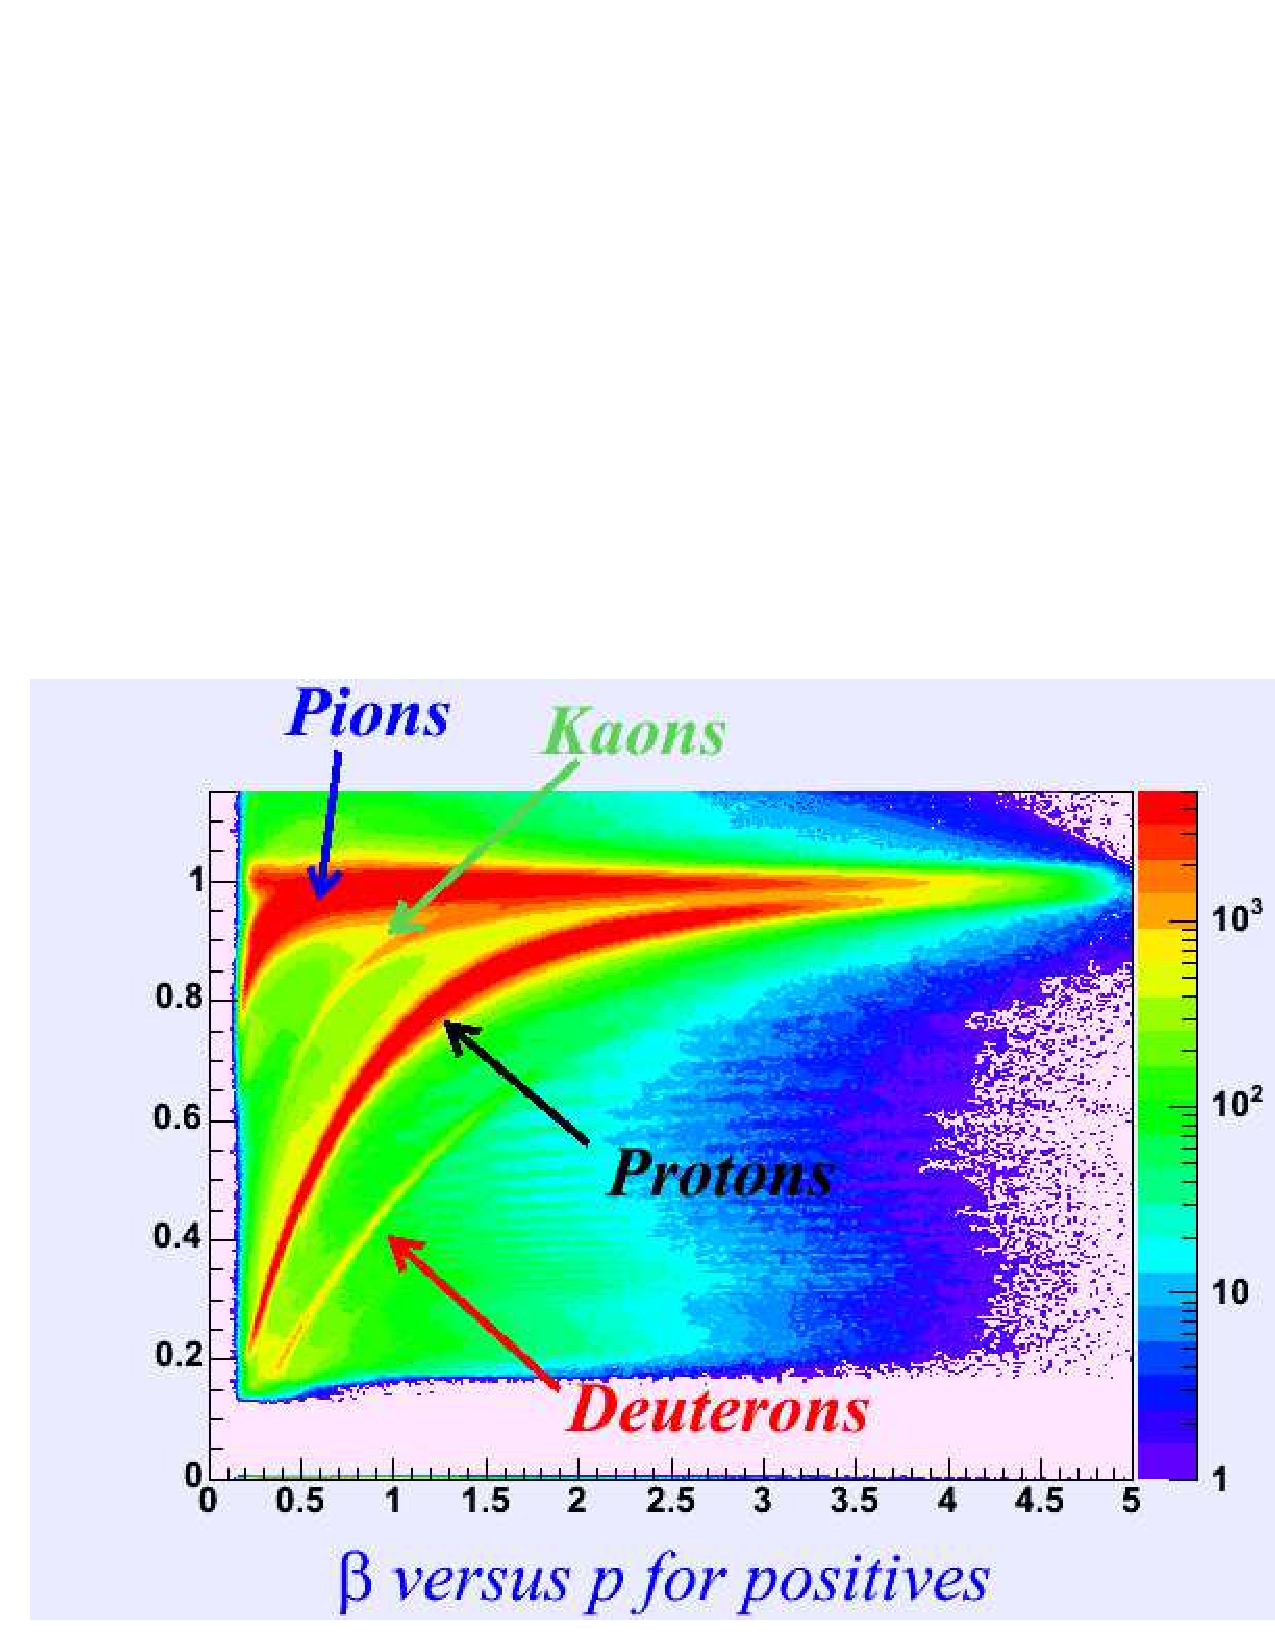
\includegraphics[width = 13cm, bb=20 0 600 740]{data_reduction/img/beta_vs_mom}
 \caption[$\beta$ versus momentum for positive particles in e1-6 running period]
         { $\beta$ versus momentum for positive particles in e1-6 running period. Bands
                    corresponding to pions, kaons, protons and deuterons are visible.}
 \label{fig:betavsmom}
\end{figure}

For the proton, the default cut is  $ 0.8 \le M \le 1.2$.
The proton ID has been redone relaxing the default cut. 
Kinematic constrains will get rid of possible ambiguities between protons and 
other particles and background.

The cut used in this analysis, illustrated in \F{fig:tofmass}, is simply:
$$
 0.6 \le M \le 1.6
$$
and it is illustrated in \F{fig:tofmass}.

\begin{figure}[h]
 \begin{center}
  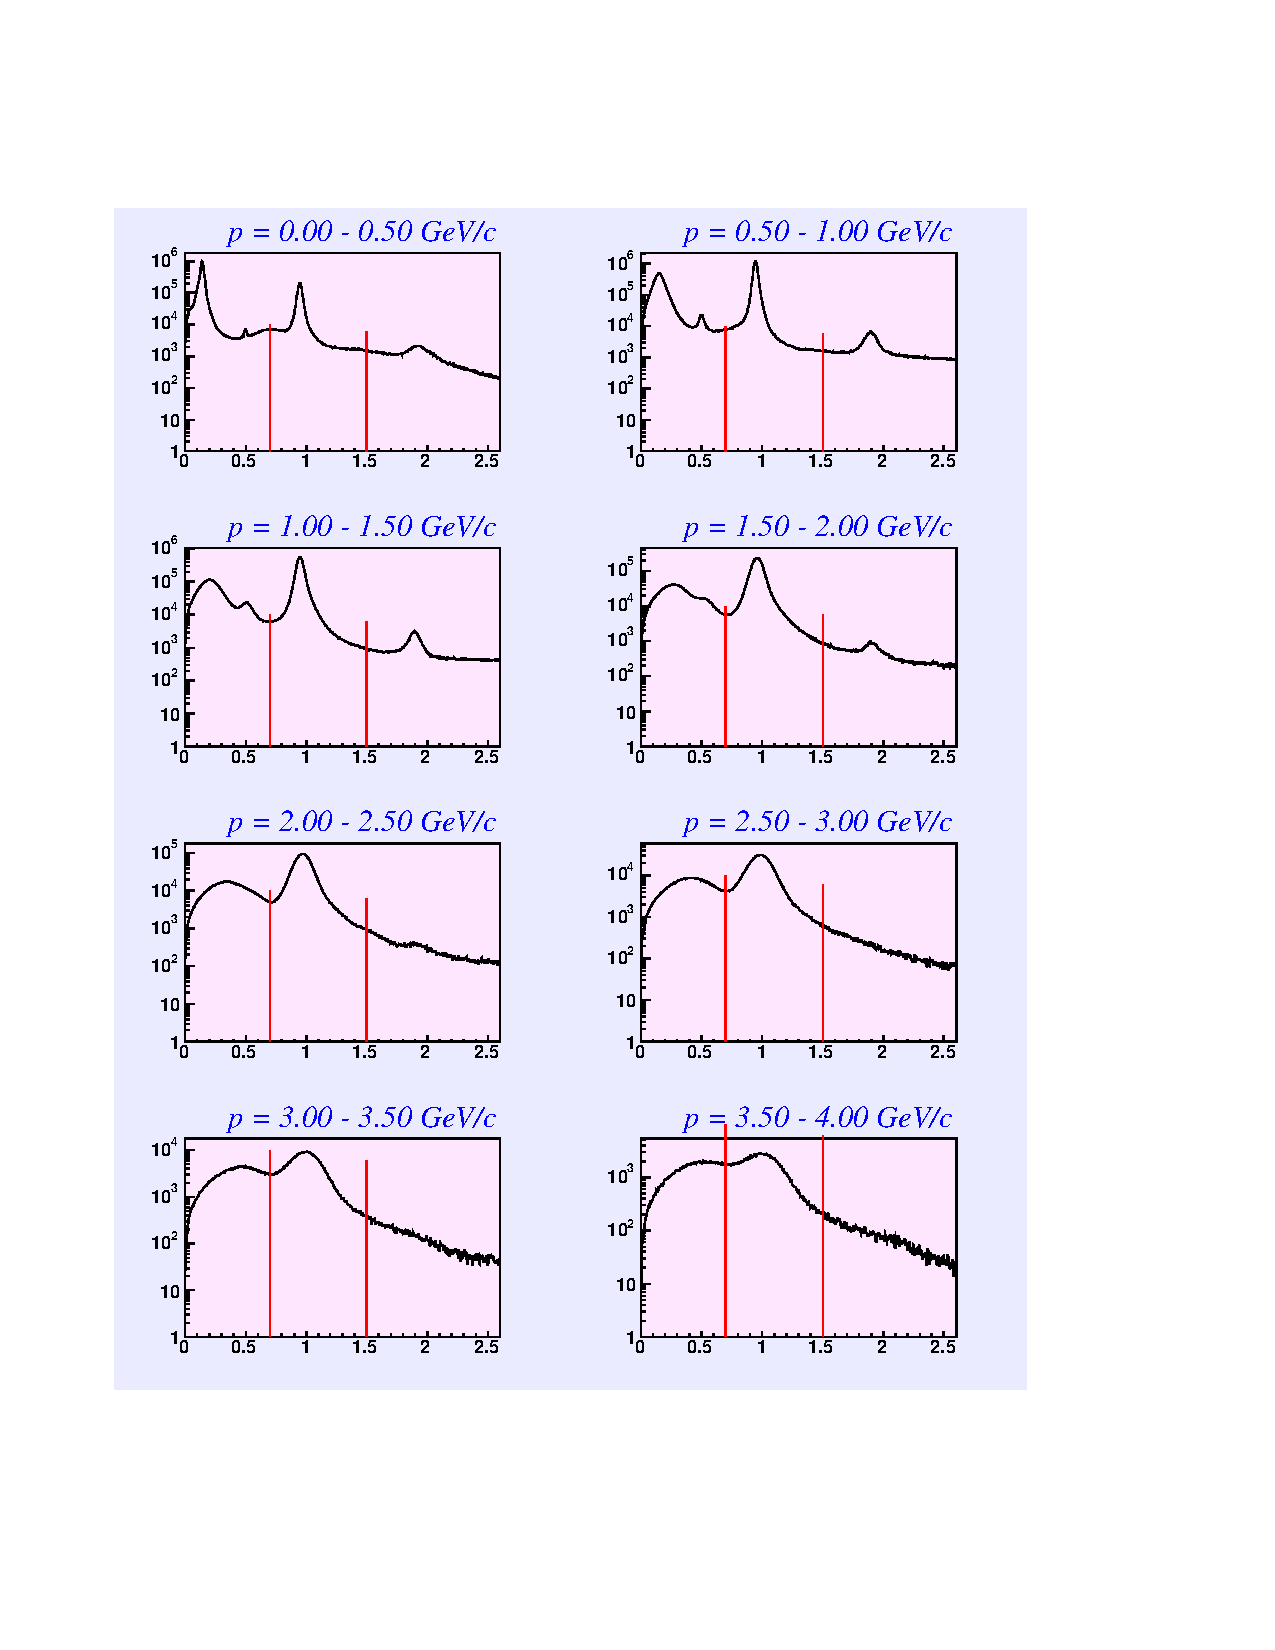
\includegraphics[width = 15cm, bb=0 120 500 750]{data_reduction/img/tof_mass}
  \caption[TOF mass spectra for CLAS]
          { TOF mass spectra for CLAS for different momemtum bins. Starting from massless particles are visible: electrons
                     (zero mass), pions, kaons, 
		     protons and finally deuterons.}
 \label{fig:tofmass}
 \end{center}
\end{figure}

